
\chapter{Time Seriers Rumor Detection Model} % (fold)
\label{cha:timr_seriers_rumor_model}
As we showed in figures \ref{fig:Url5000} and \ref{fig:largecity}, the features change during the the events' spreading over time. In order to capture these changes of the each features we use Dynamic Series-Time Structure (DSTS) which was presented in Ma's work \cite{ma2015detect}. In the an Event $E_{i}$ there is a set of tweets $tw_{ij}$ and we split them into different time intervals according to the creation time so that we can analyze the features in time series. We test the different classifiers with this model, we compare it with static features and in the end we rank all features and show their performance over time.
  \section{ Dynamic Series-Time Structure (DSTS)} 
   \subsection{Time Stamps Generation} 
   For an event $E_i$ we define $timeFirst_i$ as the start time of the event, $timeFirst_i$ as the time of last tweet of the event. We split the each tweet $tw_{ij}$ into N time intervals according to the creation time. The length of each time interval we define as follow: 
   
\begin{equation}
Interval(E_i)=\frac{\left \lceil { (timeLast_i-timeFirst_i) }\right \rceil}{N}
\end{equation}
And the index of time interval $TS(t_{ij})$ where a tweet $tw_{ij}$ which is created in time $t_{ij}$ should fall into, we define as follow :

\begin{equation}
TS(t_{ij})=\frac{\left \lfloor { (t_{ij}-timeFirst_i) }\right \rfloor}{Interval(E_i)}
\end{equation}

In our work $Interval(E_i)$ as we defined in section \ref{sec:Time_Period_of_an_Event} is one hour and N is constant 48 hours for each event.  
   
   \subsection{ Dynamic Series-Time Structure (DSTS)} 
Now we have all the time intervals of an event $E_i$ and we can generate a vector V($E_i$ ) of features in each time interval. And in order to capture the changes of feature over time we should no only model the features in individual time intervals but also we should model their difference between two time intervals. So the model of  DSTS is represented as:  

\begin{equation}
 V(E_i)=(\textbf{F}^D_{i,0}, \textbf{F}^D_{i,1},..., \textbf{F}^D_{i,N},\textbf{S}^D_{i,1},..., \textbf{S}^D_{i,N})
\end{equation}
where the $\textbf{F}^D_{i,t}$ is the feature vector in time interval t of event $E_i$.  $\textbf{S}^D_{i,t}$ is the difference between $\textbf{F}^D_{i,t}$ and $\textbf{F}^D_{i,t+1}$. V($E_i$ ) is the time series feature vector of the event $E_i$.
\begin{equation}
\textbf{F}^D_{i,t}=(\widetilde{ f}_{i,t,1},\widetilde{ f}_{i,t,2},...,\widetilde{ f}_{i,t,D})
\end{equation}

\begin{equation}
\textbf{S}^D_{i,t}=\frac{\textbf{F}^D_{i,t+1}-\textbf{F}^D_{i,t}}{Interval(E_i)}
\end{equation}
We use Z-score to normalize feature values which is implemented by sklearn.
\begin{equation}
\widetilde{f}_{i,t,k}=\frac{f_{i,t+1,k}-\overline{f}_{i,k}}{\sigma(f_{i,k})}
\end{equation}
where $f_{i,t,k}$ is the k-th feature in time interval t of the event $E_i$ in time interval t. $\overline{f}_{i,k}$ is the mean of the feature k of the event $E_i$ and $sigma(f_{i,k})$ is the standard deviation of the feature k over all time intervals. We skip this step when we use random forest and Decision Trees because they do not need feature normalization.

  \section{ Features} 
 
 We use a collection of features based on previous works  
\cite{castillo2011information}\cite{gupta2014tweetcred} \cite{yang2012automatic}\cite{liu2015real}\cite{madetecting}\cite{mendoza2010twitter}\cite{ma2015detect}\cite{wu2015false}\cite{jin2013epidemiological}. We extracted totally 50 features in table \ref{tab:full_features}. These features are not only extracted from Twitter interface but also other website like bluecoat.com we mentioned them in section \ref{cha:Data_Collection}. 
\subsection{Text Features}

\subsection{Twitter Features}
\subsection{User Features}
The list of large city \footnote{http://www.demographia.com/db-worldua.pdf}
\subsection{Epidemiological Modeling Features}
Jin's work is as far as we know the first people using epidemiological model to analyze rumors' prorogation on twitter \cite{jin2013epidemiological}. They fits the volume of the rumors and news events into two models SIS (Susceptible, Infected, Susceptible) and SEIZ (susceptible, exposed, infected, skeptic). 

\textbf{SIS} is one of the most popular epidemiological model. To adapt to the scenario of Twitter, we define a user who posts a tweet of relevant event as \textbf{(I)} infected, a user who didn't we define as \textbf{(S)} susceptible. But unlikely as a normal epidemiological scenario infected nodes can be cured and return to be susceptible,  the user once posts a tweet of the certain events, he will be classified into the infected component forever. He can't be return susceptible class. At time t the total number of population is $\Delta N(t)= I(t) + S(t)$ where $I(t)$ is the size of infected population and  $S(t)$ is the size of susceptible population.  As shown in Figure \ref{fig:SIS}, SIS model works as follow:

\begin{figure}[!h]
\center
\def\layersep{2.5cm}
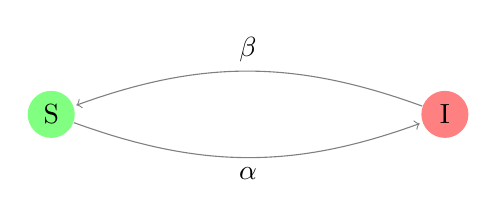
\begin{tikzpicture}[shorten >=1pt,->,draw=black!50, node distance=\layersep]
    \tikzstyle{every pin edge}=[<-,shorten <=1pt]
    \tikzstyle{neuron}=[circle,fill=black!25,minimum size=17pt,inner sep=0pt]
    \tikzstyle{input neuron}=[neuron, fill=green!50];
    \tikzstyle{output neuron}=[neuron, fill=red!50];
    % Draw the input layer nodes
     % This is the same as writing \foreach \name / \y in {1/1,2/2,3/3,4/4}
      \node[input neuron] (S) at (0,-1) {S};
     \node[ output neuron,  xshift=5cm,yshift=-1cm] (I) {I};
      \path  (I) edge [above, bend right=20]node [sloped,midway,above] {$\beta$} (S) ;
     \path  (S) edge [below, bend right=20] node [sloped,midway,below]{$\alpha $}(I) ;
    % Annotate the layers
 \end{tikzpicture}
   \caption{SIS Model}
\label{fig:SIS}
\end{figure}
	
\begin{itemize}
\item A user who posts tweets about the certain event is regarded as infected.
\item A susceptible user has not tweeted about the certain event
\item A susceptible user may see the a tweet about the certain event from a infected users and he immediately retweets or posts a tweet about this events, and in that he turns himself to infected.
\item Susceptible user will remain susceptible until he contacts (via tweet) with infected person.
\end{itemize}
we show SIS model mathematical as follow:
\begin{equation}
\frac{d[S]}{dt}=- \beta SI+\alpha I
\end{equation}
\begin{equation}
\frac{d[I]}{dt}= \beta SI-\alpha I
\end{equation}

SIS model assumes that a susceptible user once exposed to a infected user turns to infected immediately. That is one reason of this model why it didn't fit to Twitter. If fact when twitter users see a tweet they have their normal senesce to judgment the truth of the information and they can decide wether  further spreading the tweet or ignoring them.

Another popular model is SIR which contains one more term than the SIS. The definitions of \textbf{(S)} and \textbf{(I)} are the same of SIS but the term \textbf{(R)} stands for recover. Once a susceptible user is recover, he will be removed from the susceptible component and he can't be infected again. But we can't get a reasonable explanation of the term R if we model the an event spreading on Twitter.

Because of the Shortcomings of above two model, they test another model called SEIZ which reference from \cite{bettencourt2006power} . 
\begin{figure}[!h]
\center
\def\layersep{2.5cm}
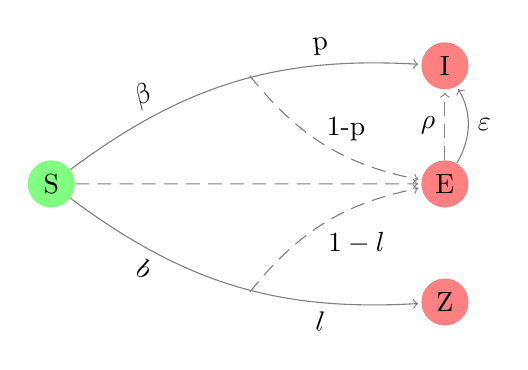
\begin{tikzpicture}[shorten >=1pt,->,draw=black!50, node distance=\layersep]
    \tikzstyle{every pin edge}=[<-,shorten <=1pt]
    \tikzstyle{neuron}=[circle,fill=black!25,minimum size=17pt,inner sep=0pt]
    \tikzstyle{input neuron}=[neuron, fill=green!50];
    \tikzstyle{output neuron}=[neuron, fill=red!50];
    \tikzstyle{miss node}=[inner sep=0,minimum size=1];
    % Draw the input layer nodes
     % This is the same as writing \foreach \name / \y in {1/1,2/2,3/3,4/4}
      \node[input neuron] (S) at (0,-2.5) {S};
      \node[ output neuron,  xshift=5cm,yshift=-1cm] (I) {I};
      \node[ output neuron,  xshift=5cm,yshift=-2.5cm] (E) {E};
      \node[ output neuron,  xshift=5cm,yshift=-4cm] (Z) {Z};
       \node[ miss node,  xshift=2.5cm,yshift=-1.1cm] (X) {};
       \node[ miss node,  xshift=2.5cm,yshift=-3.9cm] (X2) {};

	\path  (X) edge [dash pattern=on5pt off3pt,below, bend right=20] node [midway,right,xshift=-0.1cm,yshift=0.2cm]{1-p}(E) ;
 
      \path  (S) edge [above, bend left=20]node [sloped,near start,above] {$\beta$} node [sloped,near end,above] {p}  (I) ;
      \path  (E) edge [right, bend right=30] node [midway,right]{$\varepsilon $}(I) ;
      \path  (E) edge [dash pattern=on5pt off3pt] node [midway,left]{$\rho$}(I) ;
      \path  (S) edge [dash pattern=on5pt off3pt]  (E) ;
      \path  (S) edge [above, bend right=20]node [sloped,near start,below] {$b$} node [sloped,near end,below] {$l$}  (Z) ;
	\path  (X2) edge [dash pattern=on5pt off3pt,below, bend left=20] node [xshift=0.4cm]{$1-l $}(E) ;
	\end{tikzpicture}
   \caption{SEIZ Model}
\label{fig:SEIZ}
\end{figure}
\newpage
 To adapt to Twitter context, the compartments of the SEIZ model can be mapped like this: \textbf{(S)} Susceptible is a user who has not been exposed to the event aka he didn't see any tweets about the certain event yet, \textbf{(I)} infected  means a user has posted tweets about the certain events, \textbf{(Z)} skeptic is a user who has been exposed to the certain event but he decides to ignore it and \textbf{(E)} exposed is a user who been exposed to the certain event but he will post the tweets after some delay.
 
 We show the model in figure \ref{fig:SEIZ}. And the SEIZ works as follow:
 

 \begin{itemize}
\item People recruit from \textbf{(S)} Susceptible compartment to Skeptics with rate b. But with probability l some of them directly deny the events and turn to \textbf{(Z)} skeptic compartments. Others  with probability 1-l probability turn to \textbf{(E)} exposed compartment.
\item People recruit from \textbf{(S)} Susceptible compartment to Infected with rate $\beta$. But with probability p some of them directly believe the events and repost it and turn them to be \textbf{(Z)} skeptic compartments. Others  with probability 1-p probability turn to \textbf{(E)} exposed compartment.
\item  People from \textbf{(E)} exposed compartment have $\rho$ probability contacting again with the Infected and turn them to \textbf{(I)} infected compartment. And others have $\varepsilon$ probability turn into \textbf{(I)} infected compartment by themselves for example external shock.
\end{itemize}



And we show the model mathematical like:
we show SEIZ model mathematical as follow:
\begin{equation}
\frac{d[S]}{dt}=- \beta S\frac{I}{N}- b S\frac{Z}{N}
\end{equation}
\begin{equation}
\frac{d[E]}{dt}=(1-p)\beta S\frac{I}{N}+(1-l) b S\frac{I}{N}-\rho  S\frac{Z}{N}-\varepsilon E
\end{equation}
\begin{equation}
\frac{d[I]}{dt}=p\beta S\frac{I}{N}+\rho  S\frac{Z}{N}+\varepsilon E
\end{equation}
\begin{equation}
\frac{d[Z]}{dt}=lbS\frac{Z}{N} 
\end{equation}

\begin{table*}[!h]
 \centering
\scalebox{1}{
\begin{tabular}{@{\textbf{ }}lllllll@{}}
\toprule
\textbf{Symbol} & \textbf{Definition} \\ \midrule
$\beta$ & S-I contact rate\\  
b	&	 S-Z contact rate\\
$\rho $	&	E-I contact rate\\ 
$\varepsilon $   &	Incubation rate\\
$1/ \varepsilon $   &	Average Incubation Time\\
bl	&	Effective rate of S -> Z\\ 
$\beta \rho$   &	Effective rate of S -> I\\
b(1-l) & Effective rate of S -> E via contact with Z\\
$\beta (1-p)$	&	 Effective rate of S -> E via contact with I\\ 
l   &	 S->Z Probability given contact with skeptics\\
1-l &  S->E Probability given contact with skeptics\\
p	&	S->I Probability given contact with adopters\\
1-p	&	S->E Probability given contact with adopters \\ \bottomrule
\end{tabular}}
\caption{Parameters of SEIZ}
\label{tab:SEIZ_Para}
\end{table*}
\newpage
The author presents an index of SEIZ called $R_{SI}$ as equation \ref{RSI}. It contains all rate values of SEIZ and related to the flux ratio of the \textbf{(E)} exposed compartment, the ratio of entering \textbf{(E)} to leaving \textbf{(E)}. If $R_{SI}$ is bigger than 1 means the influx of exposed compartment is bigger than the efflux. This index may be a good candidate of feature to analyze rumor spreading on Twitter.


\begin{equation}
\label{RSI}
R_{SI}=\frac{(1-p)\beta+(1-l)b}{\rho+\varepsilon}  
\end{equation}

We use Levenberg-Marquard algorithm which we present in section \ref{sec:LM} to learn the parameters of the SIS and SPEI. The fitting data is the tweet volume of the 260 events  (130 rumors and 130 news). 
 In time each interval from $t_0$ to $t_n$, we fit the sequenced  tweet volume from the beginning time the $t_0$ to the current time interval $t_n$ of an event to SIS and SEIZ model and learn. From SIS we get two feature $\beta_{n},\alpha_{n}$ and from SEIZ we get 7 features $\beta_{n},b_{n},l_{n},p_{n},\varepsilon_{n},\rho_{n},RSI_{n}$. We add them into our DSTS.
 
$FittingFunction_{SIS}(TweetVolume_{0},...,TweetVolume_{n})$->$\beta_{n},\alpha_{n}$%


$FittingFunction_{SEIZ}(TweetVolume_{0},...,TweetVolume_{n})$->$\beta_{n},b_{n},l_{n},p_{n},\varepsilon_{n},\rho_{n},RSI_{n}$

 We show 4 examples as following two rumors in figure \ref{fig:SIS-rumor1} \ref{fig:SIS-rumor2} and two news in figure \ref{fig:SIS-news1}  \ref{fig:SIS-news2}. It is obvious that SEIZ is more appropriate than SIS to model in our Twitter application, because the fitting error of SPEI is less than SIS. 


\begin{figure}[!h]

  \centering

\subfigure[SIS and SEIZ model for rumor 1]{\label{fig:SIS-rumor1}
\centering
  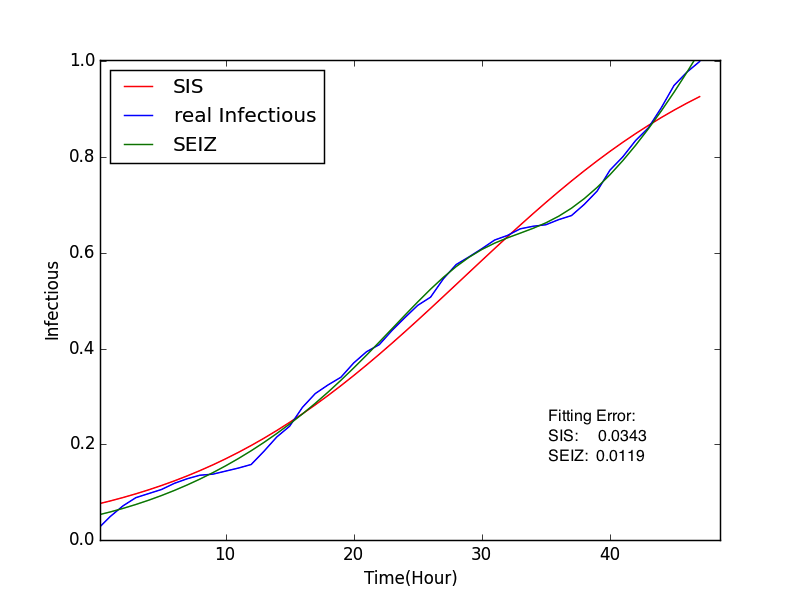
\includegraphics[width=0.48\columnwidth]{images/SISKKK.png}
} %
\subfigure[SIS and SEIZ model for rumor 2]{\label{fig:SIS-rumor2}
\centering
  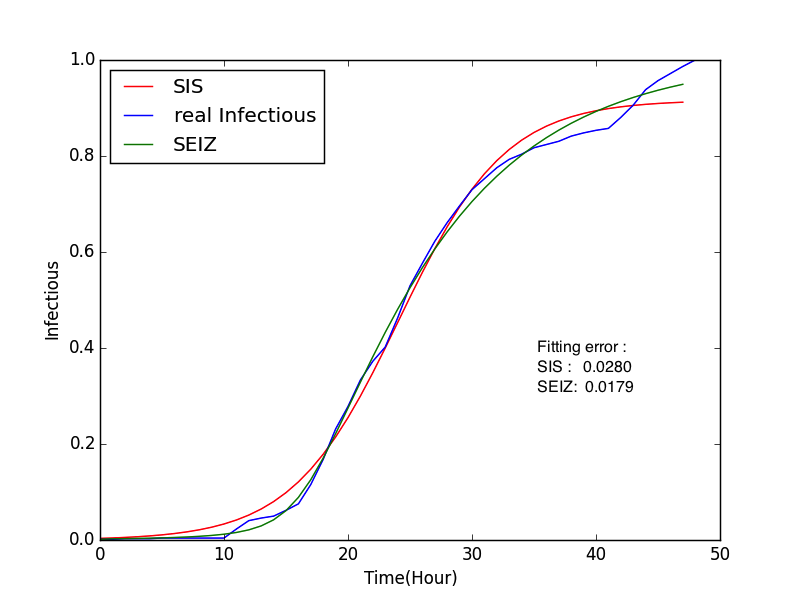
\includegraphics[width=0.48\columnwidth]{images/SIS449.png}
}
\subfigure[SIS and SEIZ model for news 1]{\label{fig:SIS-news1}
\centering
  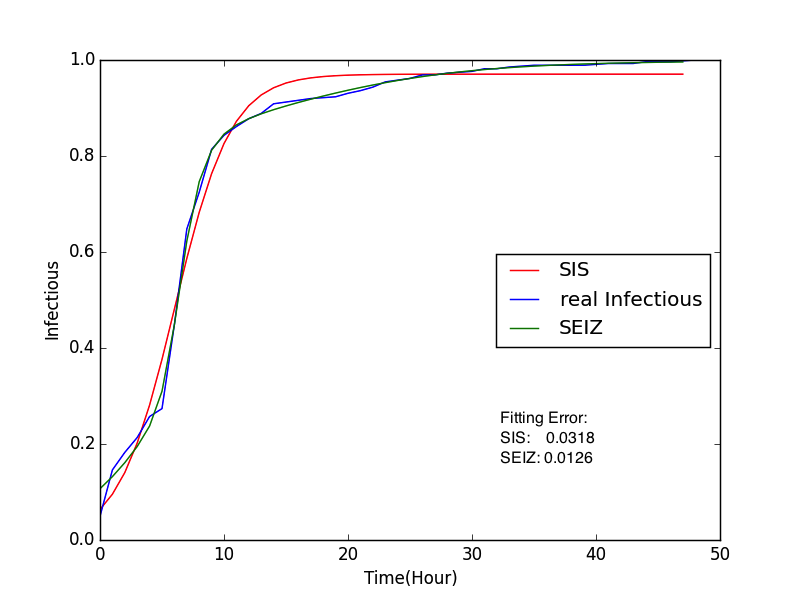
\includegraphics[width=0.48\columnwidth]{images/SISSHUMA.png}
}
\subfigure[SIS and SEIZ model for news 2]{\label{fig:SIS-news2}
\centering
  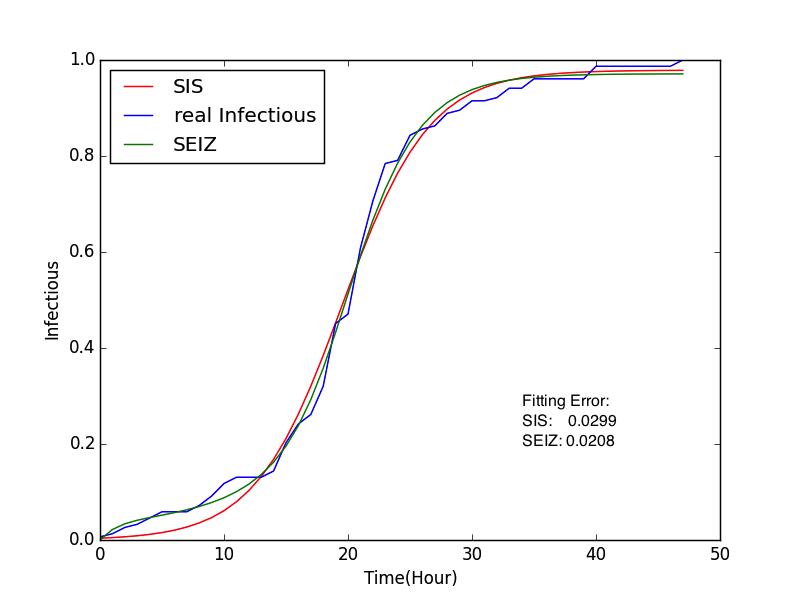
\includegraphics[width=0.48\columnwidth]{images/SIS1347.png}
}
\caption{Fitting results of SIS and SEIZ model of (a) Rumor: Robert Byrd was a member of KKK (b) Rumor: CNN altered a photograph of a shooter making him look white (c) News: Doctor announces Michael Schumacher is making process (d) News: Two U.S. sailors are arrested over an alleged rape of a Japanese woman on Okinawa}
\label{fig:SISModel}
\end{figure}

 
But fitting the models needs enough input data. We don't have enough data to learn the parameters at the first few hours. We show the performance of fitting these two model with only the first 10 hours tweet volume in figure \ref{fig:SISModelshort}. As we can see excepting the first one, the fitting result of other three is not good enough.

\begin{figure}[!h]

  \centering

\subfigure[SIS and SEIZ model for rumor 1 with 10 hours data]{\label{fig:SIS-rumor1}
\centering
  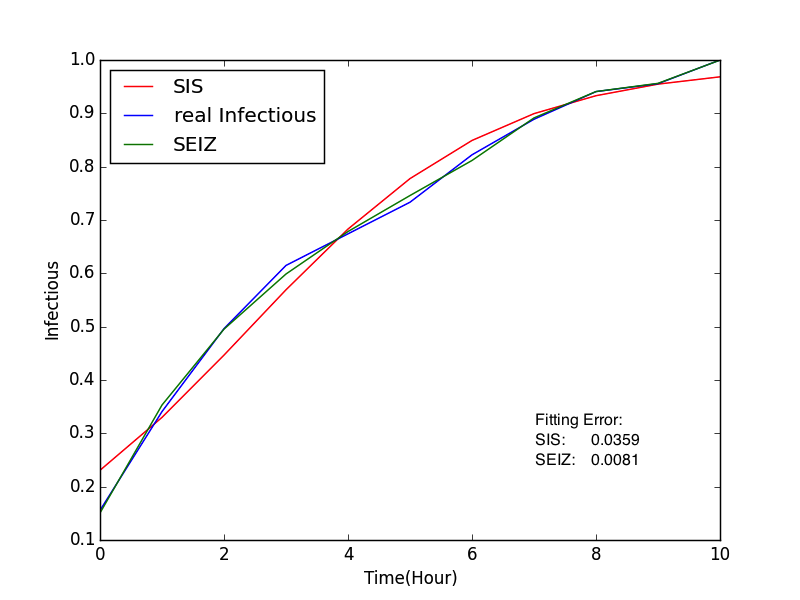
\includegraphics[width=0.48\columnwidth]{images/SISKKKshort.png}
} %
\subfigure[SIS and SEIZ model for rumor 2 with 10 hours data]{\label{fig:SIS-rumor2}
\centering
  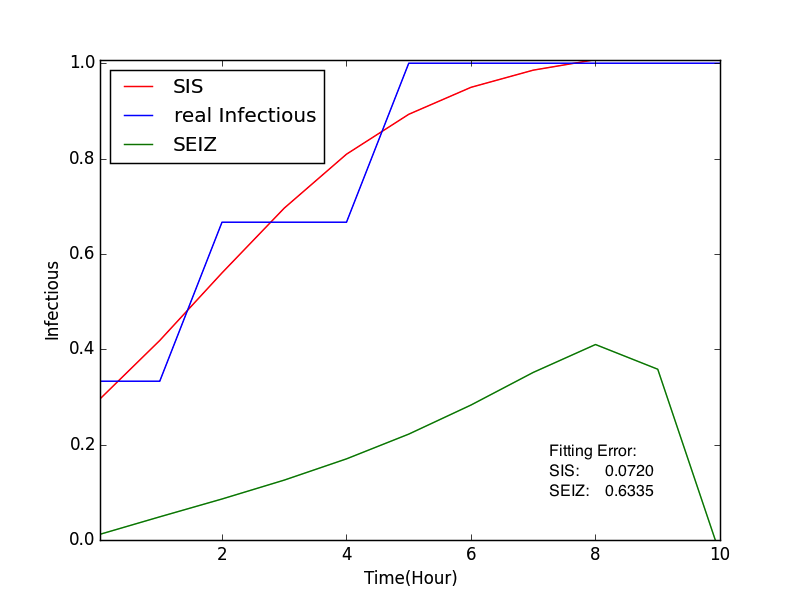
\includegraphics[width=0.48\columnwidth]{images/SIS449short.png}
}
\subfigure[SIS and SEIZ model for news 1 with 10 hours data]{\label{fig:SIS-news1}
\centering
  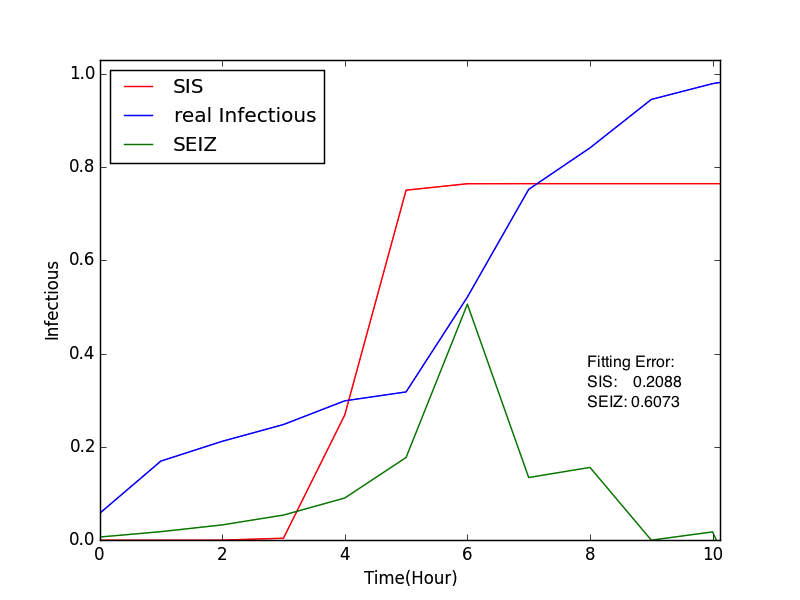
\includegraphics[width=0.48\columnwidth]{images/SISSHUMAshort.png}
}

\subfigure[SIS and SEIZ model for news 2 with 10 hours data]{\label{fig:SIS-news2}
\centering
  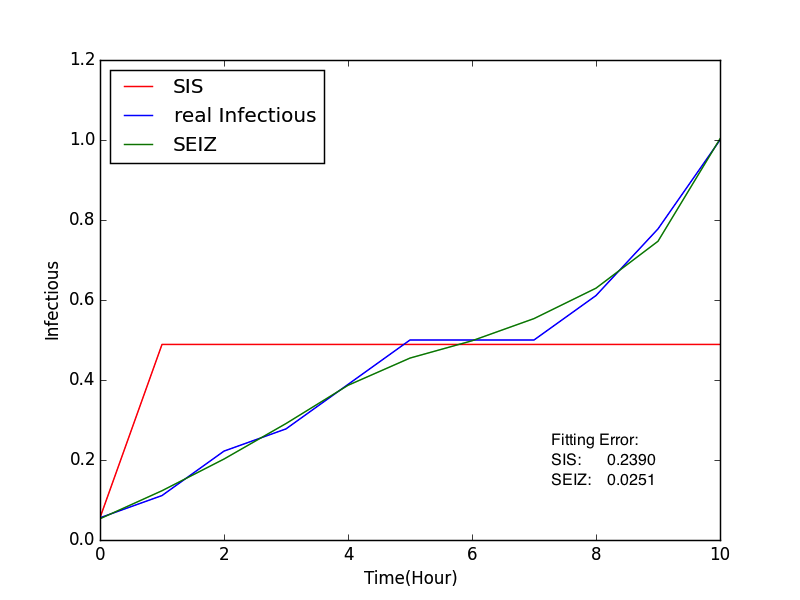
\includegraphics[width=0.48\columnwidth]{images/SIS1347short.png}
}
\caption{Fitting results of SIS and SEIZ model with only first 10 hours tweet volume data (same 4 stories as above)}
\label{fig:SISModelshort}
\end{figure}


\clearpage
\subsection{SpikeM model Features}
Kwon is another approach \cite{kwon2013prominent} discussing differences between the rumors' propagation pattern and the news events' propagation pattern on twitter. He adjusted the SpikeM Model and also used the parameters as features. 

SpikeM first was introduced by Yasuko Matsubara \cite{conf/kdd/MatsubaraSPLF12} which cab describe the pattern of information diffusion. We present it as follow:

\begin{equation}
\Delta B(n + 1) =p(n + 1)\cdot( U(n) \cdot  \sum ^n_{t=n_b}(\Delta B(t) + S(t))\cdot f(n+1-t) + \varepsilon )
\end{equation}
\begin{equation}
\label{periodic}
p(n) = 1-\frac{1}{2}P_a(\sin (\frac{2\pi}{P_p} (n+P_s)))+1)
\end{equation}

\begin{equation}
U(n + 1)=U(n)-\Delta {B(n + 1) }
\end{equation}
where
\begin{equation}
\label{decay}
f(\tau)=\beta \cdot \tau ^{-1.5}
\end{equation}
and initial conditions:
\begin{equation}
 \Delta B(0)=0 ,U(0) = N
\end{equation}
In addition, adding an external shock $S(n)$, a spike generated
at beginning time $n_b$. Mathematically, it is defined as follows:
\begin{equation}
\label{outs}
S(n) =\begin{cases}0 &(n \neq n_b)\\S_b  & (n =n_b)\end{cases} 
\end{equation}
As the definition: 
\begin{equation}
B(n) + U(n) = N
\end{equation}
The term of $\sum ^n_{t=n_b}(\Delta B(t) + S(t))$ is the total number of informed users at time n, so $\Delta B(n + 1) =p(n + 1)\cdot( U(n) \cdot  \sum ^n_{t=n_b}(\Delta B(t) + S(t))\cdot f(n+1-t) + \varepsilon )$ means that at time n+1 an infected node n randomly select a node m of all nodes and if the node m is susceptible the probability of m turning to infected is $\beta$, so it is a standard SI model. SpikeM extends the SI model from 


 \begin{itemize}
\item a power-law decay term $f(\tau)=\beta \cdot \tau ^{-1.5}
$ in equation \ref{decay}. So the earlier infected nodes has less strength of infection in a power-law decay pattern. 


\item a periodic interaction function in equation \ref{periodic}. It stands for that people have a periodic interaction patterns, like people go to sleep at night so they post much more tweets in the day. Parameters $P_p$, $P_a$, and $P_s$ are the period, strength, and shift of the periodic interaction function.
\item $\varepsilon$ is the background noise term. 
\end{itemize}
\begin{table*}[!h]
 \centering
\scalebox{1}{
\begin{tabular}{@{\textbf{ }}lllllll@{}}
\toprule
\textbf{Symbol} & \textbf{Definition} \\ \midrule
N & total population of available bloggers\\ \midrule
$n_d$	&	duration of sequence\\
n	&	time-tick (n=0, . . . , $n_d$)\\\midrule
U(n)   &	count of \textbf{\underline{u}}n-informed bloggers\\
B(n)   &	count of informed \textbf{\underline{b}}loggers\\
$\Delta B(n)$	&	count of informed \textbf{\underline{b}}loggers at time n\\\midrule
f(n)   &	in\textbf{\underline{f}}ectiveness of a blog-post, at age n\\
$\beta$ & strength of infection\\
$\beta \cdot N$	&	"first-burst" size of infection\\\midrule
S(n)   &	volume of external \textbf{\underline{s}}hock at time n\\
$n_b$ & starting time of \textbf{\underline{b}}reaking news\\
$S_b$	&	strength of external shock at birth (time $n_b$)\\
$\varepsilon$	&	background noise \\\midrule
$P_a$ & strength of periodicity\\
$P_p$			& period\\
$P_s$			& phase shift of periodicity\\ \bottomrule

\end{tabular}}
\caption{Parameters of SpikeM}
\label{tab:Features_Impsortance}
\end{table*}
But the SpikeM can't fit to the events with multi-pike like the figure \ref{fig:KKK_part}. So the author think the term external shock $S(n)$ in equation \ref{outs} should not occur once but more. So they extend the SpikeM model by adding a periodic interaction function the term external shock $S(n)$.

\begin{equation}
\Delta B(n + 1) =p(n + 1)\cdot( U(n) \cdot  \sum ^n_{t=n_b}(\Delta B(t) +  \bar{S}(t))\cdot f(n+1-t) + \varepsilon )
\end{equation}
\begin{equation}
\label{periodic}
p(n) = 1-\frac{1}{2}P_a(\sin (\frac{2\pi}{P_p} (n+P_s)))+1)
\end{equation}

\begin{equation}
U(n + 1)=U(n)-\Delta {B(n + 1) }
\end{equation}
\begin{equation}
\label{decay}
f(\tau)=\beta \cdot \tau ^{-1.5}
\end{equation}
The external shock $S(n)$ is added a a periodic interaction function
\begin{equation}
\label{outs}
\bar{S}(t)=S(t)+q(t)
\end{equation}
\begin{equation}
q(t) =  q_a(\sin (\frac{2\pi}{q_p} (t+q_s)))+1)
\end{equation}


\begin{table*}[!h]
 \centering
\scalebox{1}{
\begin{tabular}{@{\textbf{ }}lllllll@{}}
\toprule
\textbf{Symbol} & \textbf{Definition} \\ \midrule
$q_a$ & strength of periodicity of the external shock\\
$q_p$			& period of periodicity of the external shock\\
$q_s$			& phase shift of periodicity of the external shock\\ \bottomrule

\end{tabular}}
\caption{New Parameters of extended SpikeM}
\label{tab:Features_Impsortance2}
\end{table*}
\newpage
As the same approach of fitting SIS model, we learn the parameters of SpikeM model with Levenberg-Marquard algorithm. We fit the sequenced tweet volume from the beginning time the $t_0$ to the current time interval $t_n$ of an event to the model and use the output parameters as the features adding into DSTS. We use the $p_a$,  $p_p$, $p_s$ and $q_a$, $q_p$, $q_s$ as feature. We show 4 examples of the SpikeM fitting result in figure \ref{fig:SPikeModel}. But same problem as fitting SIS or SEIZ, if we test only within 10 hours data the result seems much worse than the result with full 48 hours showing in figure \ref{fig:SpikeMModelshort}.

\begin{figure}[!h]

  \centering

\subfigure[SIS and SEIZ model for rumor 1]{\label{fig:SPikeM-rumor1}
\centering
  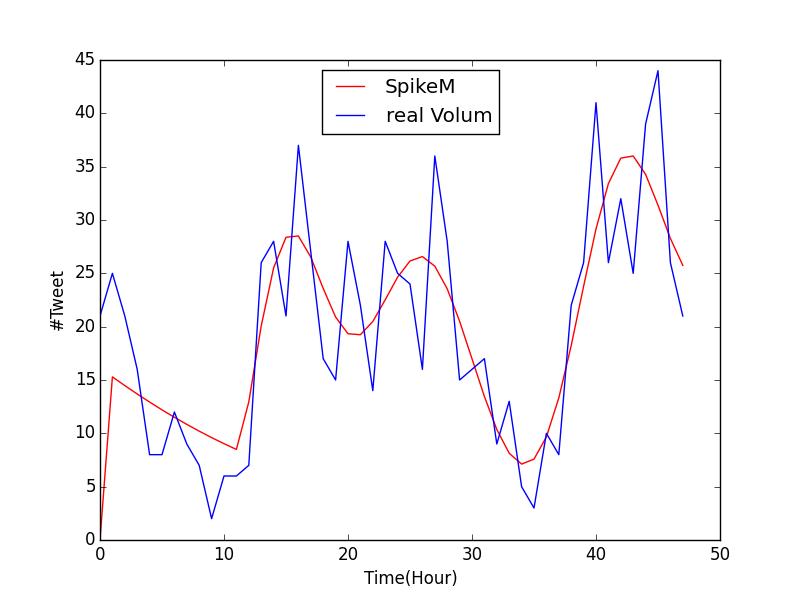
\includegraphics[width=0.48\columnwidth]{images/SpikeM_kkk.png}
} %
\subfigure[SIS and SEIZ model for rumor 2 ]{\label{fig:SPikeM-rumor2}
\centering
  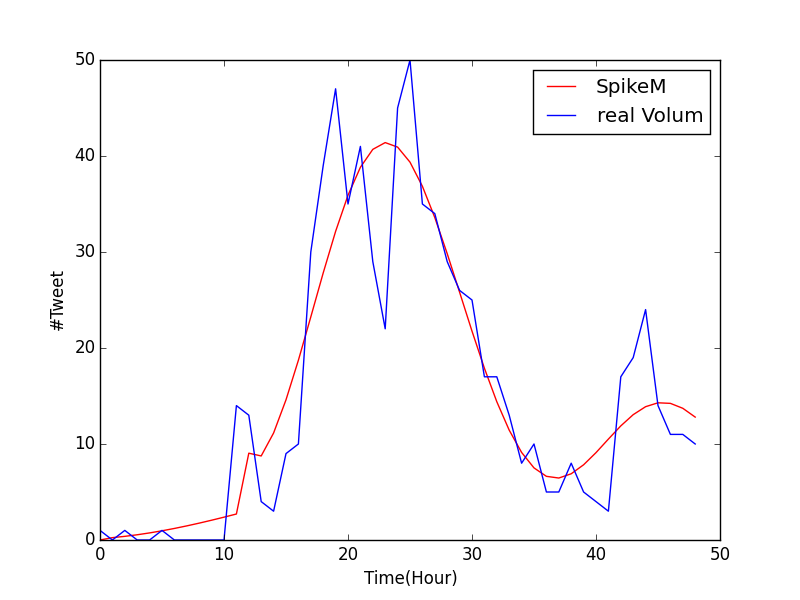
\includegraphics[width=0.48\columnwidth]{images/SpikeM_449.png}
}
\subfigure[SIS and SEIZ model for news 1]{\label{fig:SPikeM-news1}
   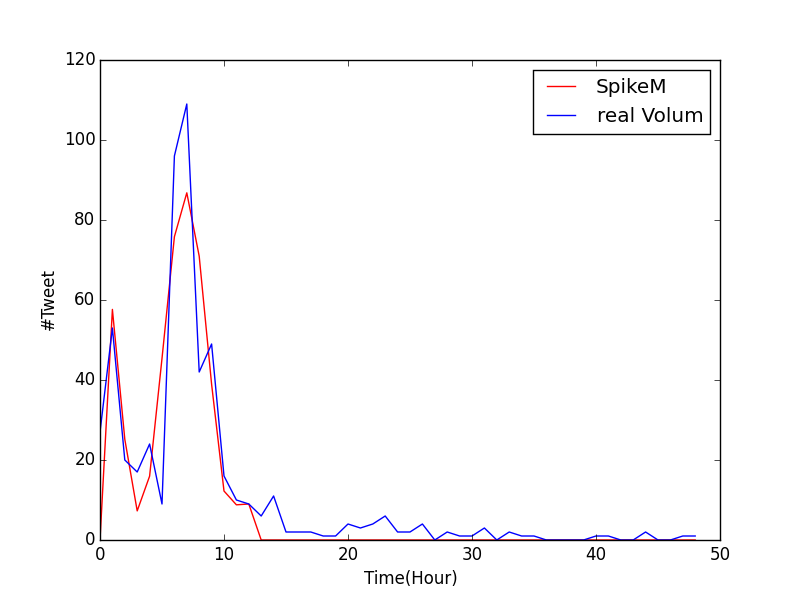
\includegraphics[width=0.48\columnwidth]{images/SpikeMSchuma.png}
}

\subfigure[SIS and SEIZ model for news 2 ]{\label{fig:SPikeM-news2}
   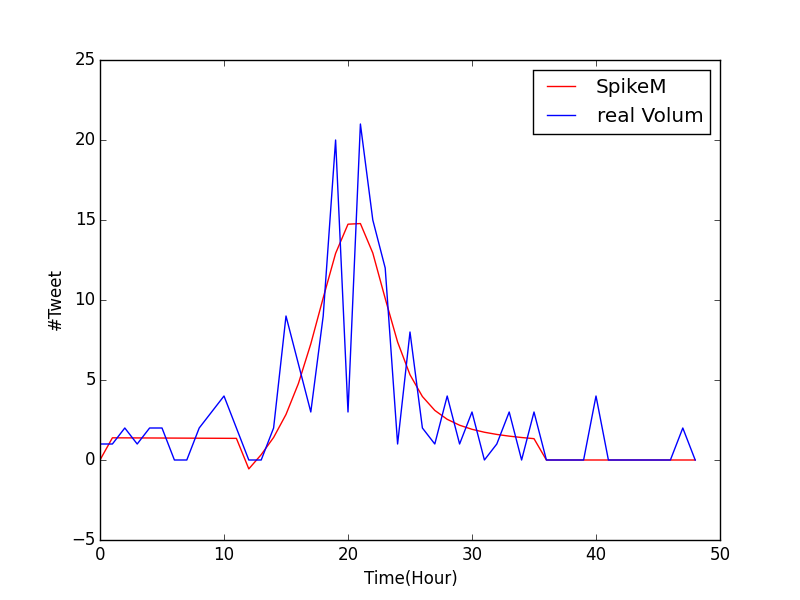
\includegraphics[width=0.48\columnwidth]{images/SpikeM_1347.png}
}
\caption{Fitting results of SpikeM model of (a) Rumor: Robert Byrd was a member of KKK (b) Rumor: CNN altered a photograph of a shooter making him look white (c) News: Doctor announces Michael Schumacher is making process (d) News: Two U.S. sailors are arrested over an alleged rape of a Japanese woman on Okinawa }
\label{fig:SPikeModel}
\end{figure}

\begin{figure}[!h]

  \centering

\subfigure[SIS and SEIZ model for rumor 1 with 10 hours data]{\label{fig:SPikeM-rumor1}
\centering
  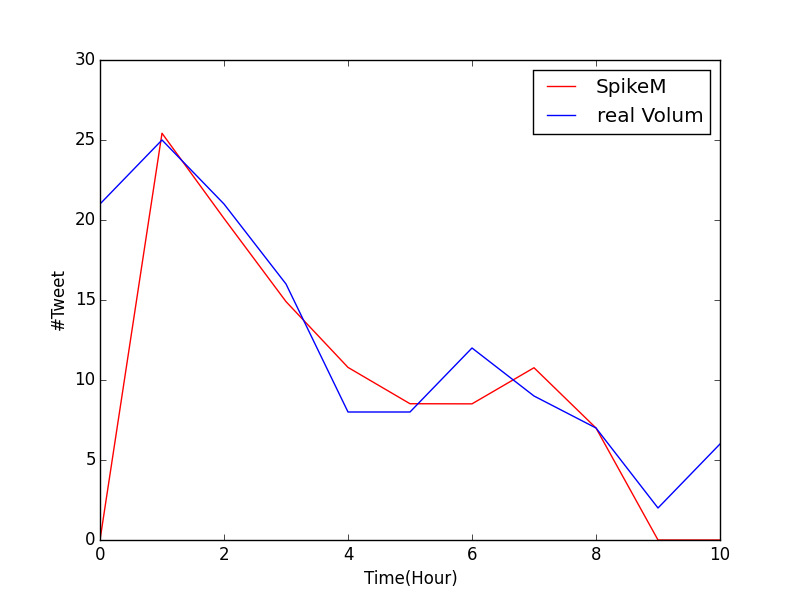
\includegraphics[width=0.48\columnwidth]{images/SpikeMKKKshort.png}
} %
\subfigure[SIS and SEIZ model for rumor 2 with 10 hours data]{\label{fig:SPikeM-rumor2}
\centering
  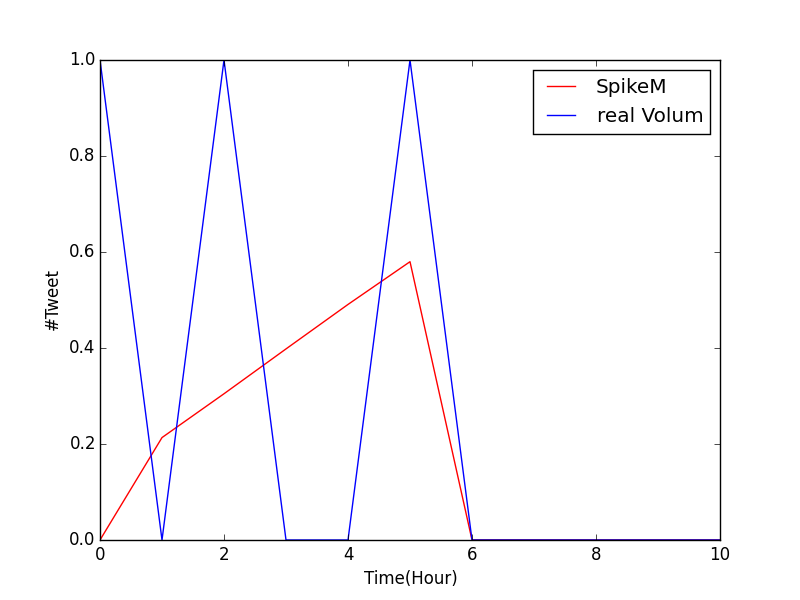
\includegraphics[width=0.48\columnwidth]{images/SpikeM492short.png}
}
\subfigure[SIS and SEIZ model for news 1 with 10 hours data]{\label{fig:SPikeM-news1}
\centering
  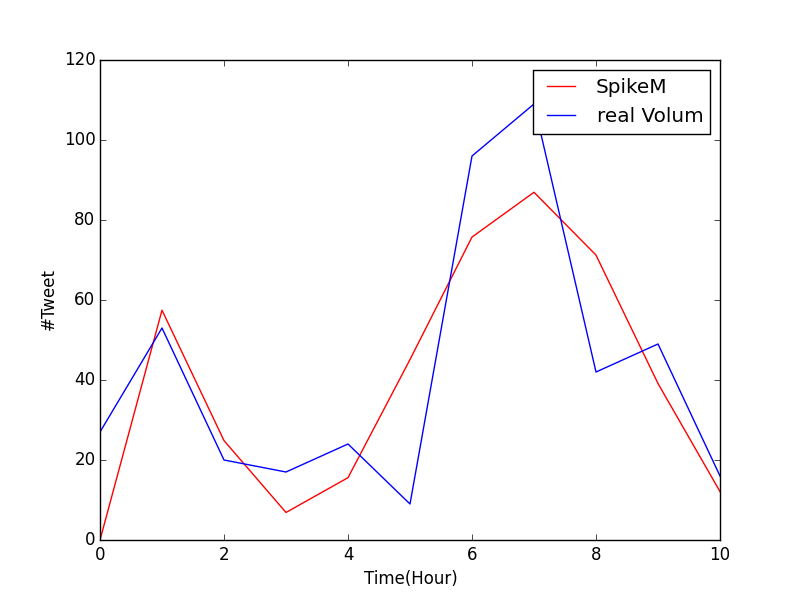
\includegraphics[width=0.48\columnwidth]{images/SpikeMSHUshort.png}
}

\subfigure[SIS and SEIZ model for news 2 with 10 hours data]{\label{fig:SPikeM-news2}
\centering
  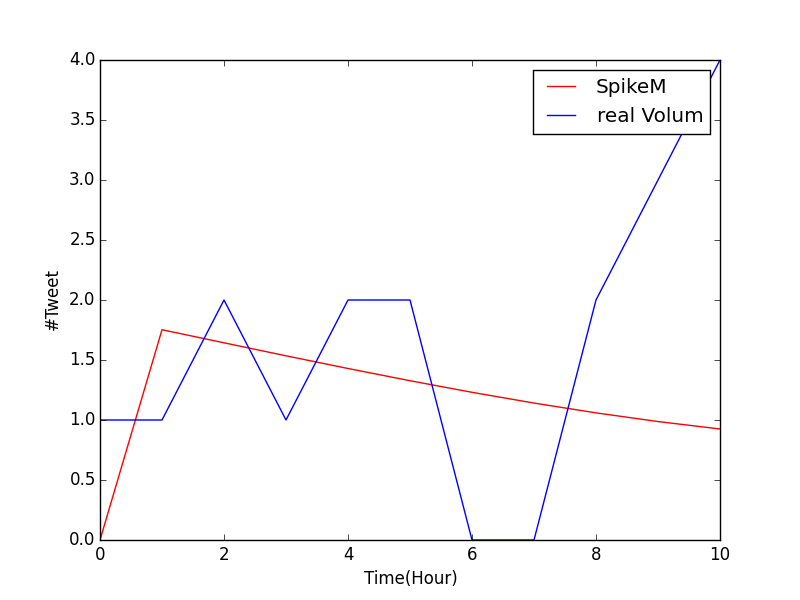
\includegraphics[width=0.48\columnwidth]{images/SpikeM1347short.png}
}
\caption{Fitting results of SpikeM model with first 10 hours data (same stories as above) }
\label{fig:SpikeMModelshort}
\end{figure}

\clearpage
\subsection{Crowd Wisdom Features}
The idea come from Liu's work \cite{liu2015real} but not same. The core idea is using the public's common sense to detecting the rumors. If there are more people denying or doubting the truth of an event, this event are more likely to be a rumor. 
In the Liu's work he uses a extensive list of positive, negative and negation keywords and a set of rules like “negative words without negation words means the poster denies the event". And he uses the ratio  number of positive  poster (supporter) to the negative poster (deny the events).

Our work is simpler than than his work. We have only a set of negative words, we call it "debunking words" like hoax, rumor, not true, etc.  In our test, this is a good feature, but it needs 17 hours to "warm up". It is logical because crowds can debunk rumors but crowds use time to react the event.

\subsection{CreditScore Features}
This feature is new feature. We our trained single tweet's creditability model the predict the tweets of the events. If the output is rumor we label it 1 otherwise 0 and we calculate the average score of the events in certain hour. We call this feature creditsScore. We will show it late, this is the best of our dataset, it improves the  performance of time series model especially in the first 12 hours. When the event begin bursting in the early stage, people can only rely on the information from the single tweet itself. Because there is no clear propagation structure (pattern) or the wise men or journalists deny the event yet. Our neural network model "sees and check" the text of a single tweet and "give us the advise" when we have no other features in the first few hours since the beginning of the events. 

The result shows this feature is the best feature.
 


\clearpage
\begin{table*}[!h]
\small
\centering
\scalebox{0.8}{
 \begin{tabular}{@{}lllllll@{}}
 \toprule
 \textbf{Category} & \textbf{Feature} & \textbf{Description}\\ \midrule
 Twitter Features& Hashtag & \% of the tweets containing \#hashtag\\
 		& Mention &  \% of the tweets mentioning others @user\\
 		& NumUrls &  \# of url in the tweet \\
 		& Retweets & average times of tweets have been retweeted \\ 
 		& IsRetweet & \% of tweets are retweeted from others\\
 		& ContainNEWS & \% of tweets containing URL and its domain's catalogue is News \\
 		& WotScore & average WOT score of domain in URL \\
 		& Isretweet & \% of tweets being retweeted from others\\
\midrule
 Text Features & LengthofTweet & average length of tweets\\
    & NumOfChar & average number of individual characters of tweets\\
   & Capital &  average fraction of characters in Uppercase of tweets \\
   & Smile & \% of tweets containing :->, :-), ;->, ;-)\\
   & Sad & \% of tweets containing :-<, :-(, ;->, ;-(\\
   & NumPositiveWords & average number of positive words\\
   & NumNegativeWords & average number of negative words\\
   & PolarityScores & average polarity scores of the Tweets\\
   & Via & \% of tweets containing via\\
   & Stock & \% of tweets containing \$ \\
   & Question & \% of tweets containing ? \\
   & Exclamation & \% of tweets containing ! \\
   & QuestionExclamation & \% of tweets containing multi Question or Exclamation mark \\ 
   & I & \% of tweets containing first pronoun like I, my, mine, we, our   \\
   & You & \% of tweets containing second pronoun like U, you, your, yours \\ 
   & HeShe & \% of tweets containing third pronoun like he, she, they, his, etc. \\ \midrule
   User Features & UserNumFollowers  & average number of followers\\
 	& UserNumFriends  & average number of friends\\
 	& UserNumTweets  & average number of users posted tweets\\
 	& UserNumPhotos  & average number of users posted photos\\
 	& UserIsInLargeCity  & \% of users living in large city\\
 	& UserJoinDate & average days since users joining Twitter\\
 	& UserDescription  & \% of user having description\\
 	& UserVerified  & \% of user being a verified user\\
 	& UserReputationScore & average ratio of \#Friends over (\#Followers + \#Friends)\\   \midrule
 Epidemiological Features & $\beta_{SIS}$ & Parameter $\beta$ of Model SIS\\
 							& $\alpha_{SIS} $ & Parameter $\alpha$ of Model SIS\\
 							& $\beta_{SEIZ}$ & Parameter $\beta$ of Model SEIZ\\
 							& $b_{SEIZ}$ & Parameter b of Model SEIZ\\
 							& $l_{SEIZ}$ & Parameter l of Model SEIZ\\
 							& $p_{SEIZ}$ & Parameter p of Model SEIZ\\
 							& $\varepsilon_{SEIZ}$ & Parameter $\varepsilon$ of Model SEIZ\\
 							& $\rho_{SEIZ}$ & Parameter $\rho$ of Model SEIZ\\
 							& $R_{SI}$ & Parameter $R_{SI}$ of Model SEIZ\\
		\midrule	
 SpikeM Model Features & $P_s$ & Parameter $P_s$ of Model Spike\\
 							& $P_a$ & Parameter $P_a$ of Model SpikeM\\
 							& $P_p$ & Parameter $P_p$ of Model SpikeM\\
 							& $Q_s$  & Parameter $Q_s$ of Model SpikeM\\
 							& $Q_a$ & Parameter $Q_a$ of Model SpikeM\\
 							& $Q_p$ & Parameter $Q_p$ of Model SpikeM\\ \midrule	
 Crowd Wisdom Features & CrowdWisdom & \% of tweets containing "Debunking Words"\\ \midrule
	 
 Credit Score Features & CreditScore & average CreditScore\\
 \bottomrule
 \end{tabular}}
 \caption{Features of Time Series Rumor Detection Model}
 \label{tab:full_features}
\end{table*}
  \section{ Classification Models } 
Same reason as the single tweet's Creditability we test the time series model also with 3 popular models Decision Trees, SVM,  Random Forest and one more model the multilayer perceptron (MLP). We show the optimized parameters in the table \ref{tab:time_model_para}. After 10-fold cross validation with same shuffled sequence  testing above models, the result is shown the figure \ref{tab:time_result}. The random forest is still the best model for our task, so we use RF as the test model for the further features' Evolution.  

\begin{table*}[!h]
 \centering
\scalebox{0.8}{
 \begin{tabular}{@{}l|l|l@{}}
 \toprule
 \multicolumn{1}{l|}{\textbf{Model}} &\multicolumn{1}{l|}{ \textbf{Parameters} }& \textbf{Value} \\ \midrule
 Random Forest & Number of Trees & 350\\ \midrule
 SVM & kernel  & radial basis function\\
 	& penalty parameter of the error term  & 3.0\\
 	& gamma  & $\frac{1}{50}$\\ \midrule
 Decision Trees & criterion & gini \\ \midrule
  MLP & alpha  & 0.0001\\
 	& activation function  & ReLU\\
 	& hidden layer sizes  & 2 layer(50 nodes each layer)\\
 	&weight optimization & adam\\ 
 \bottomrule
 \end{tabular}}
 \caption{Parameters of Classification models}
 \label{tab:time_model_para}
\end{table*}


\begin{table}[]
\centering
\begin{tabular}{|c|cccc|}
\hline
\multicolumn{1}{|c|}{\multirow{2}{*}{Model}} & \multicolumn{4}{c|}{Accuracy in hours}                     \\ \cline{2-5} 
\multicolumn{1}{|l|}{}& 6 & 12 & 24 & \multicolumn{1}{c|}{48} \\\hline
 Random Forest  & \textbf{0.8615} &  \textbf{0.8615}  &\textbf{ 0.8692} &  \textbf{0.9076 }\\
MLP & 0.7423  & 0.7423   &   0.7692   &  0.8192 \\
SVM & 0.7423  & 0.7884   &   0.7769   & 0.7538  \\
Decision Trees& 0.7807  & 0.8115   &  0.75 & 0.7385 \\    \bottomrule           
\end{tabular}
 \caption{Prediction Accuracy of Different Single Tweet's Creditability Scoring Models}
 \label{tab:time_result}
\end{table}



\newpage
  \section{ Feature Evolution } 
    \subsection{ Time Series VS Static Feature} 

First we compare our time series model and the normal static feature model. We show the result is in figure \ref{TVSF} the full 48 hours details in Appendix table \ref{TSVSSFFULL} and in figure . As we can see from the result that the accuracy of time Series is better than the static. But after 24 hours the advantage of the time series is very limited. 
 
\begin{table}[!h]
\centering
\begin{tabular}{|c|c c |c|}
\hline
Hour & Time series model & Static model & Difference \\ \hline
1    & 0.82              & 0.78         & 0.03       \\
6    & 0.86              & 0.8          & 0.06       \\
12   & 0.87              & 0.83         & 0.04       \\
18   & 0.88              & 0.83         & 0.05       \\
24   & 0.87              & 0.85         & 0.01       \\
30   & 0.88              & 0.85         & 0.03       \\
36   & 0.87              & 0.86         & 0.01          \\
42   & 0.88              & 0.88         & 0          \\
48   & 0.89              & 0.87         & 0.02      \\\hline

\end{tabular}
\caption{Accuracy: Time series VS static Features}
\label{TVSF}
\end{table}

\begin{figure}[!h]
\centering
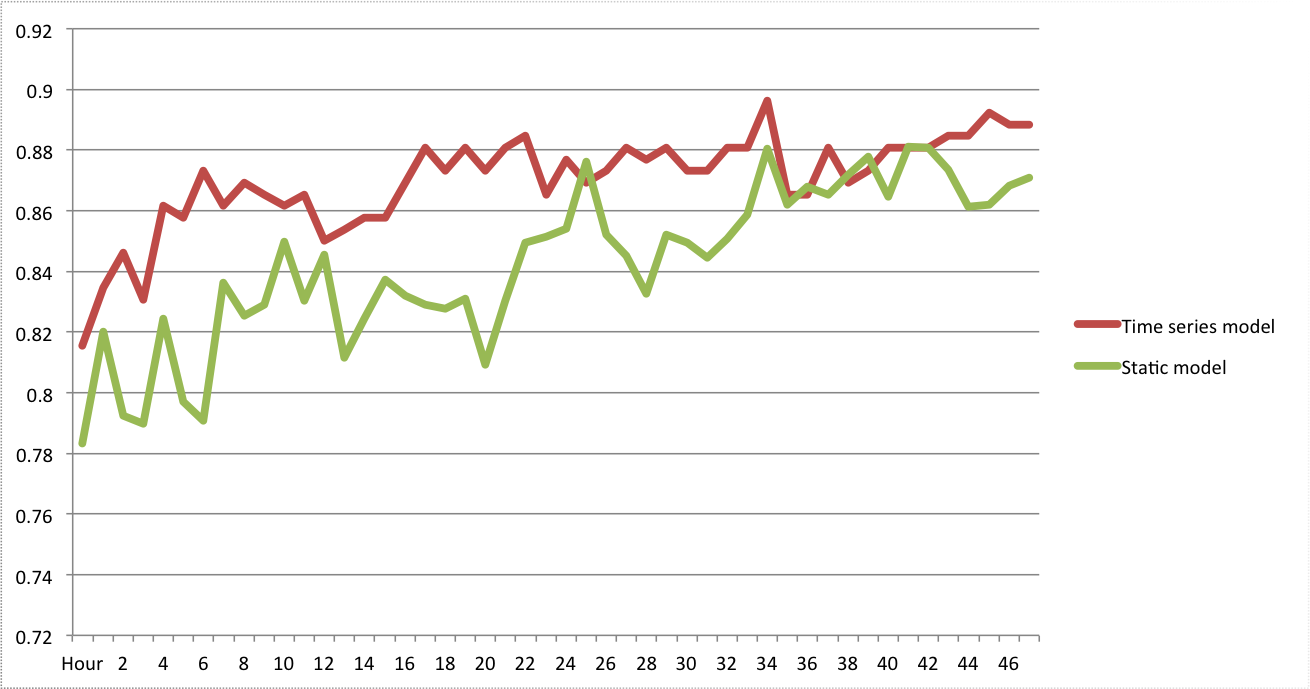
\includegraphics[width=\columnwidth]{images/Vsstatic.png}
\caption{Accuracy: Time series VS static Features}
\label{fig:TVSF}
\end{figure}

  
 \subsection{ Feature Analyzing Over Time} 
 We rank the features' importance using the method we introduced in section \ref{random_forest}, the full result is shown in Appendix table \ref{tab:allfeaturerank}.  First we split the features in 7 catalogues as table \ref{tab:full_features} Tweet\_Feature, User\_Feature,Text\_Feature,  CreditScore, SpikeM, Epidemiological Features, CrowdWisdom and the BestSets. The BestSets is top 23 features on average in table \ref{bestfeature}.
 
 \begin{table}[!h]
\centering
\begin{tabular}{|l|}
\hline
Best Feature set\\ \hline

 CreditScore \\
 ContainNEWS \\
 NumChar \\
 UserTweetsPerDays \\
 QuestionExclamation \\ 
 UserReputationScore \\

WotScore \\
Question \\
UserJoin\_date \\
Mention \\
LengthOfTweet \\
DebunkingWords \\ 
UserFollowers \\
Exclamation \\
UserVerified \\
Hashtag \\
Capital \\
You \\
UserNumPhoto \\
numUrls \\
UserFriends \\
NumPositiveWords \\
Via \\
$P_a$  \\
UserIsInLargeCity \\PolarityScores \\UserDescription \\$R_{SI}$\\$\beta_{SIS}$ \\ $\varepsilon_{SEIZ}$   \\ \bottomrule 
 \end{tabular}
\caption{Best Features}
\label{bestfeature}
\end{table}

 
 

  
  
  
